\documentclass[border=5pt]{standalone}
\usepackage{tikz}
\usepackage{amsmath}
\begin{document}
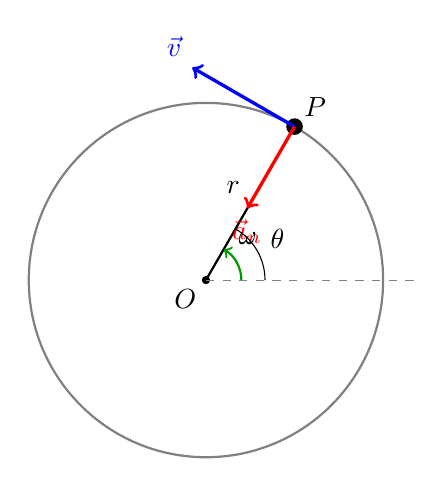
\begin{tikzpicture}[scale=1.5]
    % 圆周
    \draw[thick,gray] (0,0) circle (1.5);
    
    % 圆心
    \fill (0,0) circle (1pt) node[below left]{$O$};
    
    % 质点位置
    \coordinate (P) at (60:1.5);
    \fill (P) circle (2pt) node[above right]{$P$};
    
    % 半径
    \draw[thick] (0,0) -- (P) node[midway,above left]{$r$};
    
    % 速度矢量（切线方向）
    \draw[->,very thick,blue] (P) -- ++(150:1) node[above left]{$\vec{v}$};
    
    % 向心加速度
    \draw[->,very thick,red] (P) -- ++(240:0.8) node[below]{$\vec{a}_n$};
    
    % 角速度标注
    \draw[->,thick,green!60!black] (0.3,0) arc (0:60:0.3);
    \node at (45:0.5) {$\omega$};
    
    % 角度标注
    \draw[dashed,gray] (0,0) -- (1.8,0);
    \draw (0.5,0) arc (0:60:0.5);
    \node at (30:0.7) {$\theta$};
\end{tikzpicture}
\end{document}
